\section{互信息}
\label{sec:info-mutual-information}

公平硬币$X$经过以概率$\tfrac14$出错的线路得到$Y$。看到$Y$之前，$X$的不确定性是$\ln2$；看到$Y$以后，平均剩下$H(X\mid Y)=h_{\mathrm{b}}(\tfrac14)\approx0.562$。两者之差约$0.131$ nat，是观测$Y$平均消除的不确定性。这个差可以作为“$Y$含有多少关于$X$的信息”。

但熵之差只在熵有限、并且两个变量都是离散时才写得出来。连续变量的微分熵依赖坐标，一个变量离散、另一个连续时还会出现某一项根本没有定义的情形。本节换一个出发点：$X$与$Y$不相关联，就是联合分布等于边缘分布的乘积；联合分布偏离这个乘积的程度，用KL散度衡量。这个定义对任何取值空间都有意义，熵之差是它在条件满足时的一种算法。

\subsection{定义与独立性}
\label{sec:info-mi-definition}

先回顾第~\ref{chap:distribution-comparison}章的KL散度。设$P,Q$是同一可测空间上的概率分布。若$P\ll Q$，记$r=\mathrm{d}P/\mathrm{d}Q$，则
\begin{equation}
  D_{\mathrm{KL}}(P\Vert Q)=\int\ln r\,\mathrm{d}P\in[0,+\infty];
  \label{eq:info-kl-recall}
\end{equation}
若$P$不绝对连续于$Q$，则$D_{\mathrm{KL}}(P\Vert Q)=+\infty$。$\ln r$的负部总对$P$可积，所以积分总有意义；KL散度非负，并且为零当且仅当$P=Q$。离散时$r(x)=p(x)/q(x)$，式~\eqref{eq:info-kl-recall}化为$\sum_xp(x)\ln\frac{p(x)}{q(x)}$。

\begin{definition}[互信息]
\label{def:info-mutual-information}
设随机变量（或随机元素）$X,Y$的联合分布为$P_{X,Y}$，边缘分布为$P_X,P_Y$。$X$与$Y$的\term{互信息}（mutual information）是
\begin{equation}
  I(X;Y)=D_{\mathrm{KL}}\bigl(P_{X,Y}\Vert P_X\otimes P_Y\bigr)\in[0,+\infty].
  \label{eq:info-mutual-information}
\end{equation}
离散时
\begin{equation}
  I(X;Y)=\sum_{x,y}p_{X,Y}(x,y)\ln\frac{p_{X,Y}(x,y)}{p_X(x)\,p_Y(y)}.
  \label{eq:info-mutual-information-discrete}
\end{equation}
\end{definition}

$P_X\otimes P_Y$是“边缘不变、但把两个变量拆成独立”所得的分布。互信息比较真实的联合规律与这个独立参照，差异全部来自依赖关系，因为两者的边缘完全相同。

\begin{theorem}[互信息的基本性质]
\label{thm:info-mi-basic}
对任意随机元素$X,Y$：
\begin{enumerate}
  \item $I(X;Y)\geq0$；
  \item $I(X;Y)=I(Y;X)$；
  \item $I(X;Y)=0$当且仅当$X$与$Y$独立。
\end{enumerate}
\end{theorem}

\begin{proof}
第一条和第三条是KL散度的非负性及其零值条件：$I(X;Y)=0$当且仅当$P_{X,Y}=P_X\otimes P_Y$，而这正是第~\ref{chap:probability-spaces}章中独立的定义。

第二条用交换坐标的映射$\sigma(x,y)=(y,x)$。它把$P_{X,Y}$推前为$P_{Y,X}$，把$P_X\otimes P_Y$推前为$P_Y\otimes P_X$。若$P_{X,Y}\ll P_X\otimes P_Y$，密度为$r$，则$r\circ\sigma^{-1}$是推前后两个分布之间的密度，按推前测度的积分换元，两个KL的积分相等；若不绝对连续，推前后同样不绝对连续，两边都是$+\infty$。
\end{proof}

第三条比“协方差为零”强得多。取$X$在$\{-1,0,1\}$上均匀，$Y=X^{2}$：$\operatorname{Cov}(X,Y)=\mathbb{E}[X^{3}]=0$，但$Y$由$X$确定，下一小节会算出$I(X;Y)\approx0.637>0$。互信息为零能排除一切形式的依赖，零协方差只能排除线性部分。

\paragraph{二元例子}
用式~\eqref{eq:info-mutual-information-discrete}计算出错线路的例子。联合表是对角$\tfrac38$、非对角$\tfrac18$，边缘乘积处处$\tfrac14$，比值分别为$\tfrac32$与$\tfrac12$。于是
\[
  I(X;Y)=2\cdot\tfrac38\ln\tfrac32+2\cdot\tfrac18\ln\tfrac12=\tfrac34\ln\tfrac32-\tfrac14\ln2\approx0.1308\ \mathrm{nat},
\]
约$0.189$ bit。对角格的比值大于$1$，说明“相同”比独立时更常见；非对角格的比值小于$1$，对数为负，但按$P_{X,Y}$加权后总和非负。

\paragraph{互信息可以为无穷}
定义允许$I(X;Y)=+\infty$，这不是边缘情形。设$X\sim\operatorname{Unif}(0,1)$，$Y=X$。联合分布全部集中在对角线$D=\{(x,x)\}$上，$P_{X,Y}(D)=1$；而
\[
  (P_X\otimes P_Y)(D)=\int_0^1P_Y(\{x\})\,\mathrm{d}x=0.
\]
$P_{X,Y}$不绝对连续于$P_X\otimes P_Y$，所以$I(X;Y)=+\infty$。一个连续变量完全知道另一个连续变量，等于知道了无穷多位小数。离散时也会出现无穷：若$H(X)=+\infty$，令$Y=X$，下一小节会得到$I(X;Y)=H(X)=+\infty$。

定义也不要求任何密度。联合分布可以没有联合密度，比如上面集中在对角线上的分布；只要$P_{X,Y}\ll P_X\otimes P_Y$，KL就由密度比计算，否则直接为无穷。

\subsection{与熵的关系}
\label{sec:info-mi-entropy}

回到章首的说法：互信息是观测带来的不确定性的减少。下面的定理说明，离散情形下只要相关的熵有限，两种说法一致。

\begin{theorem}[互信息与熵]
\label{thm:info-mi-entropy}
设$X,Y$是离散随机变量。若$H(X)<\infty$，则$H(X\mid Y)\leq H(X)$，并且
\begin{equation}
  I(X;Y)=H(X)-H(X\mid Y).
  \label{eq:info-mi-entropy-difference}
\end{equation}
若$H(X)$与$H(Y)$都有限，则$H(X,Y)$有限，并且
\begin{equation}
  I(X;Y)=H(X)+H(Y)-H(X,Y).
  \label{eq:info-mi-entropy-sum}
\end{equation}
\end{theorem}

\begin{proof}
在$p_{X,Y}(x,y)>0$的点，把比值中的$p_{X,Y}/p_Y$写成条件概率，
\[
  \ln\frac{p_{X,Y}(x,y)}{p_X(x)p_Y(y)}=\bigl(-\ln p_X(x)\bigr)-\bigl(-\ln p_{X\mid Y}(x\mid y)\bigr).
\]
记$A=-\ln p_X(X)$，$B=-\ln p_{X\mid Y}(X\mid Y)$。两者非负，期望分别为
\[
  \mathbb{E}[A]=H(X)<\infty,\qquad\mathbb{E}[B]=H(X\mid Y).
\]由式~\eqref{eq:info-mutual-information-discrete}，$I(X;Y)=\mathbb{E}[A-B]$。$A$可积而$B\geq0$，期望可以拆开，得到
\[
  I(X;Y)=\mathbb{E}[A]-\mathbb{E}[B]=H(X)-H(X\mid Y).
\]
互信息非负，所以$H(X\mid Y)\leq H(X)$，右端是两个有限数之差。

第二个等式由链式法则得到：$H(Y)<\infty$时由第一部分$H(X\mid Y)\leq H(X)<\infty$，式~\eqref{eq:info-entropy-chain-rule}给出$H(X,Y)=H(Y)+H(X\mid Y)$有限，代入式~\eqref{eq:info-mi-entropy-difference}即得。
\end{proof}

由对称性，同样有$I(X;Y)=H(Y)-H(Y\mid X)$（$H(Y)<\infty$时）。这几个关系有三个直接推论，都在相应熵有限时成立：
\begin{itemize}
  \item \textbf{条件化平均不增加熵}：$H(X\mid Y)\leq H(X)$，等号当且仅当$X,Y$独立。上一节的表~\eqref{eq:info-z-table}说明，这个结论只对平均成立，对单个观测值$H(X\mid Y=0)$可以大于$H(X)$。
  \item \textbf{联合熵的次可加性}：$H(X,Y)\leq H(X)+H(Y)$，这正是图~\ref{fig:info-same-marginals}中观察到的。
  \item \textbf{上界}：$I(X;Y)\leq\min\{H(X),H(Y)\}$，并且$I(X;X)=H(X)$，因为$H(X\mid X)=0$。离散变量与自身的互信息就是它的熵，熵因此也叫“自身信息”。
\end{itemize}

$Y=X^{2}$的例子中，$Y$是$X$的函数，$H(Y\mid X)=0$，所以$I(X;Y)=H(Y)$；$Y$取$1$的概率是$\tfrac23$，$H(Y)=h_{\mathrm{b}}(\tfrac13)\approx0.637$。

\begin{BookInlineFigure}
  \centering
  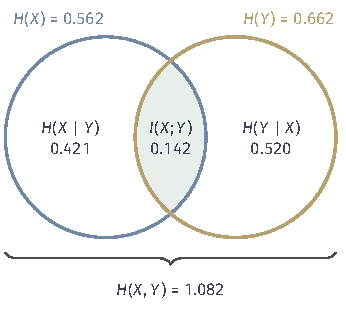
\includegraphics[width=58.5mm]{figures/07-probability/04-distribution-analysis/tikz/info-venn/figure.pdf}
  \caption{两个离散变量的熵与互信息的记账图，数值（nat）取自表~\eqref{eq:info-z-table}。蓝圈表示$H(X)$，黄圈表示$H(Y)$，重叠部分（浅绿）表示$I(X;Y)$，两圈之外的部分分别是条件熵，两圈的并表示$H(X,Y)$。图只表示有限熵之间的加减关系，面积不是测度。}
  \label{fig:info-venn}
\end{BookInlineFigure}

图~\ref{fig:info-venn}把这些关系画成两个重叠的圆。表~\eqref{eq:info-z-table}给出
\[
  I(X;Y)=H(X)-H(X\mid Y)\approx0.562-0.421=0.142,
\]
也等于$H(Y)-H(Y\mid X)\approx0.662-0.520=0.142$。图很方便记忆，但它只是有限熵之间的记账：三个变量时，三圈公共部分对应的量可以为负（第~\ref{sec:info-mi-chain-rule}节的异或例子），连续变量时各块可以为负，不能把它当成真正的面积。

再看出错线路的例子随出错概率$\varepsilon$的变化。$H(X)=\ln2$不变，$H(X\mid Y)=h_{\mathrm{b}}(\varepsilon)$，所以
\[
  I(X;Y)=\ln2-h_{\mathrm{b}}(\varepsilon).
\]
图~\ref{fig:info-bsc-curves}中两条曲线之和始终是$\ln2$。$\varepsilon=0$时观测完全揭示$X$；$\varepsilon=\tfrac12$时$Y$与$X$独立，互信息为零；$\varepsilon=1$时线路总是出错，把$Y$翻转回来就完全知道$X$，互信息又回到$\ln2$。互信息衡量的是能否从$Y$推出$X$，不是$Y$与$X$是否相等。

\begin{BookInlineFigure}
  \centering
  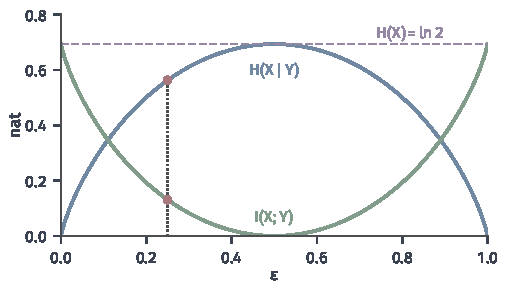
\includegraphics[width=86mm]{figures/07-probability/04-distribution-analysis/matplotlib/info-bsc-curves/figure.pdf}
  \caption{公平硬币$X$经以概率$\varepsilon$出错的线路得到$Y$。蓝线为$H(X\mid Y)=h_{\mathrm{b}}(\varepsilon)$，绿线为$I(X;Y)=\ln2-h_{\mathrm{b}}(\varepsilon)$，紫虚线为$H(X)=\ln2$，单位nat。红点为$\varepsilon=\tfrac14$：$0.562$与$0.131$。}
  \label{fig:info-bsc-curves}
\end{BookInlineFigure}

\paragraph{连续情形}
$(X,Y)$有联合密度时，若$h(Y)$与$h(Y\mid X)$都有限，同样的推导（把求和换成积分，拆开的依据是两项都绝对可积）给出
\[
  I(X;Y)=h(Y)-h(Y\mid X).
\]
二元标准正态由式~\eqref{eq:info-gaussian-entropy}与式~\eqref{eq:info-gaussian-conditional-entropy}得到
\begin{equation}
  I(X;Y)=\frac12\ln(2\pi\mathrm{e})-\frac12\ln\bigl(2\pi\mathrm{e}(1-\rho^{2})\bigr)=-\frac12\ln(1-\rho^{2}).
  \label{eq:info-gaussian-mi}
\end{equation}
$\rho=0.9$时约$0.830$ nat；$\lvert\rho\rvert\to1$时趋于无穷，与上面$Y=X$的例子一致。两个微分熵各自依赖坐标，相减后的互信息不依赖：分别把$X,Y$作伸缩，式~\eqref{eq:info-differential-entropy-scale}中的$\ln\lvert a\rvert$在两项中相消。

\begin{BookInlineFigure}
  \centering
  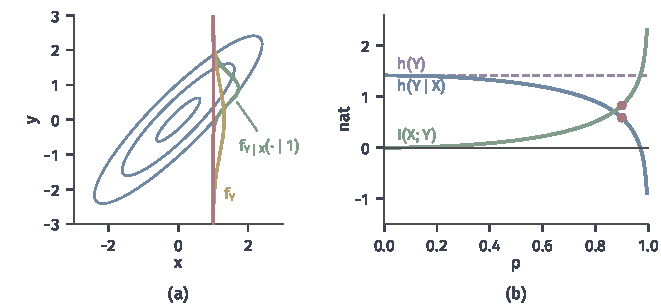
\includegraphics[width=112mm]{figures/07-probability/04-distribution-analysis/matplotlib/info-gaussian-mi/figure.pdf}
  \caption{二元标准正态分布。(a)$\rho=0.9$时联合密度的等值线（蓝）；红线为$x=1$，绿线为$Y$在$X=1$下的条件密度$\mathcal{N}(0.9,0.19)$，黄线为$Y$的边缘密度$\mathcal{N}(0,1)$，均横向画出。(b)$h(Y)$（紫虚线）、$h(Y\mid X)$（蓝）与$I(X;Y)$（绿）随$\rho$的变化，单位nat；红点为$\rho=0.9$时的$0.589$与$0.830$。}
  \label{fig:info-gaussian-mi}
\end{BookInlineFigure}

图~\ref{fig:info-gaussian-mi}(a)是熵差的直观来源：条件密度比边缘密度窄得多，宽度之比的对数就是减少的不确定性。(b)中$h(Y\mid X)$在$\rho$接近$1$时变为负数，而互信息始终非负。

熵差公式需要的熵可能不存在，互信息却仍有定义。设$X$等可能取$\pm1$，$Z\sim\mathcal{N}(0,1)$与$X$独立，$Y=X+Z$。$X$是离散的，没有密度，$h(X)$与$h(X\mid Y)$都没有定义，“$h(X)-h(X\mid Y)$”写不出来。但给定$X=x$时$Y$的条件密度是$\varphi(y-x)$，$h(Y\mid X)=\tfrac12\ln(2\pi\mathrm{e})$；$Y$的密度是两个正态密度的平均，方差为$2$，$h(Y)$有限。于是
\[
  I(X;Y)=h(Y)-h(Y\mid X)
\]
是一个有限的正数。所以，熵差是在各项有意义时计算互信息的工具，而式~\eqref{eq:info-mutual-information}才是定义。

\subsection{条件互信息}
\label{sec:info-conditional-mi}

已经知道第三个变量$Z$时，$X$与$Y$之间还剩多少共享信息？做法与条件熵相同：固定$Z=z$，在条件分布下计算互信息，再按$Z$的分布平均。连续的$Z$要用第~\ref{chap:conditional-distributions}章的正则条件分布，才能对每个$z$谈论“给定$Z=z$时$(X,Y)$的分布”。

\begin{definition}[条件互信息]
\label{def:info-conditional-mi}
设$X,Y,Z$取值于标准Borel空间，于是$(X,Y)$给定$Z$的正则条件分布$P_{X,Y\mid Z}(\cdot\mid z)$存在，记其边缘为$P_{X\mid Z}(\cdot\mid z)$、$P_{Y\mid Z}(\cdot\mid z)$。$X$与$Y$在给定$Z$时的\term{条件互信息}（conditional mutual information）是
\begin{equation}
  I(X;Y\mid Z)=\int D_{\mathrm{KL}}\bigl(P_{X,Y\mid Z}(\cdot\mid z)\Vert P_{X\mid Z}(\cdot\mid z)\otimes P_{Y\mid Z}(\cdot\mid z)\bigr)\,P_Z(\mathrm{d}z).
  \label{eq:info-conditional-mi}
\end{equation}
离散时
\begin{equation}
  I(X;Y\mid Z)=\sum_{x,y,z}p_{X,Y,Z}(x,y,z)\ln\frac{p_{X,Y\mid Z}(x,y\mid z)}{p_{X\mid Z}(x\mid z)\,p_{Y\mid Z}(y\mid z)}.
  \label{eq:info-conditional-mi-discrete}
\end{equation}
\end{definition}

被积函数是$z$的非负可测函数，积分在$[0,+\infty]$中总有意义。正则条件分布只在$P_Z$几乎处处的意义下唯一，换一个版本只在零概率的$z$上改变被积函数，积分不变。没有标准Borel这类条件时，正则条件分布可能不存在，式~\eqref{eq:info-conditional-mi}就不能这样写。

\begin{theorem}[条件互信息与条件独立]
\label{thm:info-conditional-mi-zero}
在定义~\ref{def:info-conditional-mi}的条件下，$I(X;Y\mid Z)\geq0$；$I(X;Y\mid Z)=0$当且仅当$X$与$Y$在给定$Z$时条件独立。
\end{theorem}

\begin{proof}
被积函数是KL散度，非负，所以积分非负。非负函数的积分为零，当且仅当它对$P_Z$几乎处处为零；由KL的零值条件，这就是对几乎所有$z$，
\[
  P_{X,Y\mid Z}(\cdot\mid z)=P_{X\mid Z}(\cdot\mid z)\otimes P_{Y\mid Z}(\cdot\mid z).
\]按第~\ref{chap:conditional-distributions}章，这正是给定$Z$时的条件独立。
\end{proof}

在离散且$H(X\mid Z)<\infty$时，把定理~\ref{thm:info-mi-entropy}的证明逐个条件值地做一遍，得到
\begin{equation}
  I(X;Y\mid Z)=H(X\mid Z)-H(X\mid Y,Z).
  \label{eq:info-conditional-mi-entropy}
\end{equation}
它是在已经知道$Z$的前提下，再观测$Y$所减少的关于$X$的不确定性。

条件互信息与互信息是两个不同的量，下一小节的例子说明两者之间没有固定的大小关系。

\subsection{互信息的链式法则}
\label{sec:info-mi-chain-rule}

一组观测$(Y,Z)$提供的关于$X$的信息，可以分两步获得：先看$Y$，得到$I(X;Y)$；再看$Z$，新增的是已知$Y$时$Z$还能提供的信息$I(X;Z\mid Y)$。

\begin{theorem}[互信息的链式法则]
\label{thm:info-mi-chain-rule}
设$X,Y,Z$取值于标准Borel空间，则在$[0,+\infty]$中
\begin{equation}
  I(X;Y,Z)=I(X;Y)+I(X;Z\mid Y).
  \label{eq:info-mi-chain-rule}
\end{equation}
一般地，
\begin{equation}
  I(X;Y_1,\dots,Y_n)=\sum_{i=1}^{n}I(X;Y_i\mid Y_1,\dots,Y_{i-1}).
  \label{eq:info-mi-chain-rule-n}
\end{equation}
\end{theorem}

\begin{proof}
先证离散且$H(X)<\infty$的情形。由式~\eqref{eq:info-mi-entropy-difference}及其条件形式~\eqref{eq:info-conditional-mi-entropy}，
\[
  I(X;Y,Z)=H(X)-H(X\mid Y,Z),\qquad I(X;Y)=H(X)-H(X\mid Y),
\]
以及
\[
  I(X;Z\mid Y)=H(X\mid Y)-H(X\mid Y,Z).
\]
三个式子里的熵都不超过$H(X)$，都是有限数。后两式相加，$H(X\mid Y)$相消，得到第一式。

一般情形不能假定熵有限，要直接分解KL散度。在离散情形，对一切三元组有
\[
  \frac{p_{X,Y,Z}}{p_X\,p_{Y,Z}}=\frac{p_{X,Y}}{p_X\,p_Y}\cdot\frac{p_{X,Z\mid Y}}{p_{X\mid Y}\,p_{Z\mid Y}},
\]
等式两边分子分母都按$p_{X,Y,Z}=p_{X,Y}\,p_{Z\mid X,Y}$与$p_{Y,Z}=p_Y\,p_{Z\mid Y}$展开即可核对。取对数后按$P_{X,Y,Z}$平均，第一个因子给出$I(X;Y)$，第二个给出$I(X;Z\mid Y)$。在一般空间，这一步是KL散度对联合分布的分解：两个联合分布的KL等于边缘的KL加上条件分布KL的平均。把两项的平均拆开、并允许取$+\infty$，需要用到对数比负部的可积性与正则条件分布的可测性，推导较长，这里只用它的结论。

多个观测时对$n$归纳：把$(Y_1,\dots,Y_{n-1})$看成一个变量，对它与$Y_n$用式~\eqref{eq:info-mi-chain-rule}。
\end{proof}

一般空间中KL散度分解的完整论证，读者可查阅~\scite{math-cover2006information}。

链式法则说明，信息可以按观测的先后分批记账，与熵的链式法则平行。不过，下面两个例子说明，第二步的条件互信息可以比无条件的互信息大，也可以小。

\paragraph{条件化可以增加互信息}
设$X,Y$是独立的公平硬币，$Z=X\oplus Y$为异或（相同为$0$，不同为$1$）。$X,Y$独立，$I(X;Y)=0$。给定$Z=0$时，$(X,Y)$只取$(0,0),(1,1)$，各$\tfrac12$，$Y$由$X$确定；给定$Z=1$时只取$(0,1),(1,0)$。于是
\[
  I(X;Y\mid Z)=H(X\mid Z)-H(X\mid Y,Z)=\ln2-0=\ln2.
\]
这里用到$X$与$Z$独立（$Z$在$X$的每个取值下都是公平硬币），所以$H(X\mid Z)=\ln2$；而知道$Y$与$Z$就能算出$X=Y\oplus Z$。

\begin{BookInlineFigure}
  \centering
  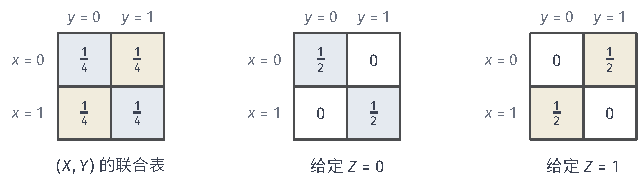
\includegraphics[width=108.6mm]{figures/07-probability/04-distribution-analysis/tikz/info-xor/figure.pdf}
  \caption{异或例子。左：独立公平硬币$(X,Y)$的联合表，蓝格$Z=X\oplus Y=0$，黄格$Z=1$。中、右：给定$Z=0$与$Z=1$后$(X,Y)$的条件表，质量只落在两格上，$Y$由$X$确定。}
  \label{fig:info-xor}
\end{BookInlineFigure}

图~\ref{fig:info-xor}给出了直观：单看$(X,Y)$，四格均匀，看不出任何关联；一旦知道$Z$，就只剩两格，$X$与$Y$紧紧绑在一起。$Z$本身不含关于$X$的信息，它提供的是$X$与$Y$之间的约束。

用链式法则从两个方向计算$I(X;Y,Z)$。先看$Y$再看$Z$：
\[
  I(X;Y)+I(X;Z\mid Y)=0+\ln2.
\]
先看$Z$再看$Y$：
\[
  I(X;Z)+I(X;Y\mid Z)=0+\ln2.
\]
两种顺序都给出$\ln2$：单独看$Y$或$Z$都毫无用处，两者合起来却完全确定$X$。

\paragraph{条件化可以减少互信息}
设$X$是公平硬币，$Y=Z=X$。则$I(X;Y)=H(X)=\ln2$；给定$Z$以后$X,Y$都已确定，$I(X;Y\mid Z)=0$。这次$Z$与$Y$携带的是同一份信息，知道$Z$以后，$Y$不再提供新东西。

两个例子放在一起说明，“三圈公共部分”$I(X;Y)-I(X;Y\mid Z)$在异或例子中等于$-\ln2$，在复制例子中等于$\ln2$。图~\ref{fig:info-venn}那样的记账图不能推广到三个变量的面积图，条件化前后的互信息要分别计算。
